\section{Cherenkov Detectors \cite{cherenkov}}
Cherenkov detectors are based on the fact that charged particles that travel faster than light in a medium emit light. This light can be used to reconstruct properties of the particles.
\subsection{Theoretical principles}
\begin{wrapfigure}{l}{0.31\textwidth}
    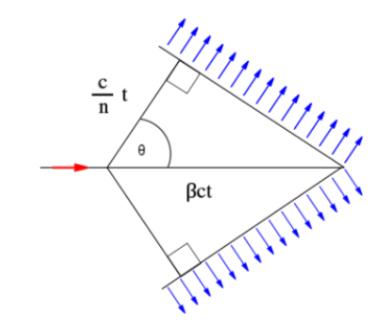
\includegraphics[width=0.3\textwidth]{graphics/Cone.png}
    \caption{Schematic representation of the Cherenkov light cone. \cite{cherenkov}}
  \end{wrapfigure}
  \FloatBarrier
The speed of light in a medium is given by $c = \frac{c_0}{n}$, where $c_0$ is the speed of light in vacuum and $n$ the refractive index of the medium. If a charged particle travels localy with $v_p > c$, it emits Cherenkov photons under an angle $\vartheta$. This is caused by the relaxation of the polarization of a dielectric medium. Due to the high velocity of the particle an aysymmetric polarization of the medium is created, which then leads to a Mach cone. The angle is given by
\begin{align*}
  \cos \vartheta = \frac{c/n \, t}{\beta\, c\, t} = \frac{1}{n \, \beta} \, .
\end{align*}
The cherenkov radiation has a continuous spectrum with a maximum in the UV range. The intensity is approximately proportional to the frequency of the light in the visible spectrum. This is the reason why Cherenkov radiation is usually seen as blue.\\
For Cherenkov light in the atmosphere there are usually two different sources. The first cone is produced by the original particle e.g. an iron nucleus and the second one by the particle shower produced due to the original particle.
\subsection{Historical development}
Pawel Cherenkov discovered the light around a radioactive preparation in water in 1934. I. Tamm and I. Frank developed the corresponding theory in 1937. All theorists were awarded with the Nobel prize for their work in 1958. The first Cherenkov counter was developed in 1951 and was used to detect cosmic rays with Cherenkov light in water. A cylinder with distilled water was used as the radiator. The Cherenkov light was measured via a photomultiplier and matching preamplifier to increase the signals.
Around the same time a so called getting type Cherenkov detector was designed. The radiator was an acrylic plastic cone with a top angle $\Phi$. It was followed by a lens that only focusses Cherenkov light that was emitted with $\vartheta = \Phi$ through a collimeter, which was measured by a photomultiplier afterwards.
\subsection{Cherenkov detector types}
\textit{Threshold Detectors} were used in earlier collider experiments starting in 1951. They used specific mediums to distinguish different particles. The produced photons were beamed towards photomultipliers by using mirrors. The peak height measured with the photomultiplier could be used to reconstruct the particle's velocity. They made it possibe to distinguish between pions, kaons and protons.
\textit{Differential Cherenkov Detectors} use the angle of the Cherenkov cone together with a spherical mirror to focus the light trough a diaphragm. The radius of the diaphragm limits the measurable velocity range. Changing the pressure inside of the gas radiator controlls the refractive index. For this reason they are used to select particles instead of identifying them.\\
\textit{Ring Imaging Cherenkov Detectors} (RICH) were first designed in 1976. They can be used to reconstruct the particle'section speed between $0.5-\SI{150}{\giga\electronvolt}$. At higher momenta it is not possible to distinguish the Cherenkov angles of different particles. They consist of a sperical detector ($R_c$) surrounded by a mirror ($R$) while the radiator is filled in between.

\begin{wrapfigure}{l}{0.5\textwidth}
    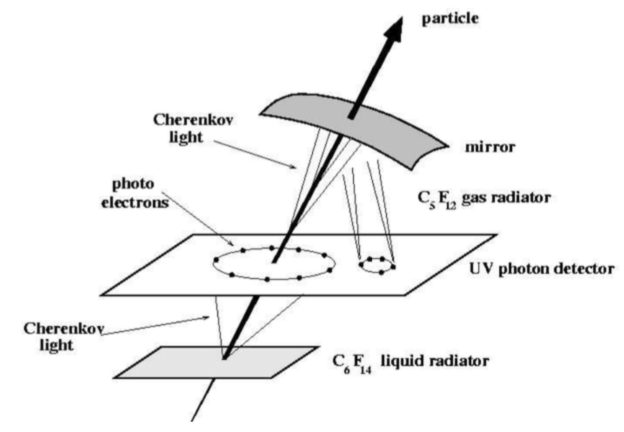
\includegraphics[width=0.48\textwidth]{graphics/RICH.png}
    \caption{RICH detector in the DELPHI experiment using two radiators and one photon detector. The Cherenkov light is projected on both sides of the detector. \cite{cherenkov}}
		\label{fig:RICH}
  \end{wrapfigure}
  \FloatBarrier

The Cherenkov light is emitted in between the detector and the mirror and reflected onto the photo detector. This reflection makes it possible to calculate the velocity with $\vartheta \approx 2\frac{R_c}{R}$. Current RICH detectors work with two radiators leading to a larger momentum range as shown in figure \ref{fig:RICH}.
The main challenge for the photo detector is that it must be able to localize the spatial positions in the ring image. The Cherenkov photons are transformed into photoelectrons and measured in a multiwire propotional chamber. This leads to the reconstruction of two coordinates, where one can be calculated from the drift time of the electrons. \textit{Detection of Internally Reflected Cherenkov light} (DIRC) is a principle utilizing a pipe radiator to produce the Cherenkov light and guide it towards a light catcher. The angle information remains unchanged. This detector type was used in the Babar experiment \textit{Cherenkov Calorimeter} for example made out of lead glass as a radiator. The produced light is propotional to the energy of the entering charged particles. This technology was used for the electromagnetic calorimeter of the OPAL experiment as well.\\
The first \textit{Imaging Atmospheric Cherenkov Telescope} was developed by the Whipple collaboration in the early 1980s. They were able to detect the Cherenkov light of particle showers created by high energy cosmic gamma and proton rays. These showers create Cherenkov light when travelling through the atmosphere, which the Whipple telescope could detect in a range of \SI{50}{\giga\electronvolt} to \SI{50}{\tera\electronvolt}. A large segmented, spherical mirror was used to reflect the Cherenkov light onto an array of photomultipliers. Gamma showers are usually of elliptic shape when projected to the ground, while hadronic interactions result in broader and irregular showers due to the larger transverse momenta of the generated particles. Usually the Cherenkov cones cover a size of several $\SI{100}{\meter}^2$; therefore several telescopes are grouped together to cover as much of the shower as possible. A benefit of this is, that the angular resolutions increaseswith each added telescope. Furthermore, projecting all images into one plane allows for a betetr reconstruction of the source position by using stereoscopic features. IACT detectors were for example used for to the observation of the Crab nebula, the brightest steady source observable on earth, in 1989. Until today they provide the best measurements of angular and energy spectra in the \si{\tera\electronvolt} domain.\\
A special use of IACT detectors are \textit{Neutrino Observatories}. The IceCUBE experiment located at the Amundsen-Scott South Pole Station in Antarctica consists of 86 photomultipliers that are symmetricly placed incide of a $\SI{1}{\kilo\meter}^3$ cube of ice. The ice functions as a radiator. If a neutrino reacts within the ice, it creates charged leptons that can radiate Cherenkov light. On the surface of the cube a detector with the purpose to detect cosmic particles is located, called IceTop. These detections can then be used as a veto to filter as many atmospheric neutrinos from the data as possible. The DeepCore is build out of the 6 most inner photomultipliers, which are placed in a smaller distance from another. This is the reason why IceCUBE measures neutrinos in the range of \SI{100}{\giga\electronvolt} to several \si{\peta\electronvolt}. Besides the reconstruction of the energy it is also possible to determine the original direction of the neutrinos. IceCUBE measured a non-terrestrial neutrino flux in 2013. One of the most recent discoveries were the identification of two high-energy neutrino sources. Another neutrino observatory is located in Japan. It is calles Super-Kamiokande and is a cylindrical water tank with a volume of around $\SI{200000}{\meter}^3$. It is placed \SI{1}{\kilo\meter} below the surface and uses the same principles as IceCUBE does with the antarctic ice. Here the photomultipliers are positioned at the walls of the tank. Electrons travelling through the water produce a spheric Cherenkov ring, while the track of muons is much longer due to the slower energy loss. One of the most important discoveries of the Super-Kamiokande experiment was the discovery of neutrino oszillation.
